\documentclass{article}%
\usepackage[T1]{fontenc}%
\usepackage[utf8]{inputenc}%
\usepackage{lmodern}%
\usepackage{textcomp}%
\usepackage{lastpage}%
\usepackage[head=40pt,margin=0.5in,bottom=0.6in]{geometry}%
\usepackage{graphicx}%
%
\title{\textbf{Mosquiteros impregnados de medicamento contra paludismo}}%
\author{AFP}%
\date{04/03/2019}%
%
\begin{document}%
\normalsize%
\maketitle%
\textbf{URL: }%
http://www.eluniversal.com/estilo{-}de{-}vida/34351/mosquiteros{-}impregnados{-}de{-}medicamento{-}contra{-}paludismo\newline%
%
\textbf{Periodico: }%
EU, %
ID: %
34351, %
Seccion: %
estilo{-}de{-}vida\newline%
%
\textbf{Palabras Claves: }%
NO\_TIENE\newline%
%
\textbf{Derecho: }%
2.1%
, Otros Derechos: %
\newline%
%
\textbf{\textit{Esta herramienta estaría contribuyendo a la prevención de las picaduras de mosquitos que portan la enfermedad}}%
\newline%
\newline%
%
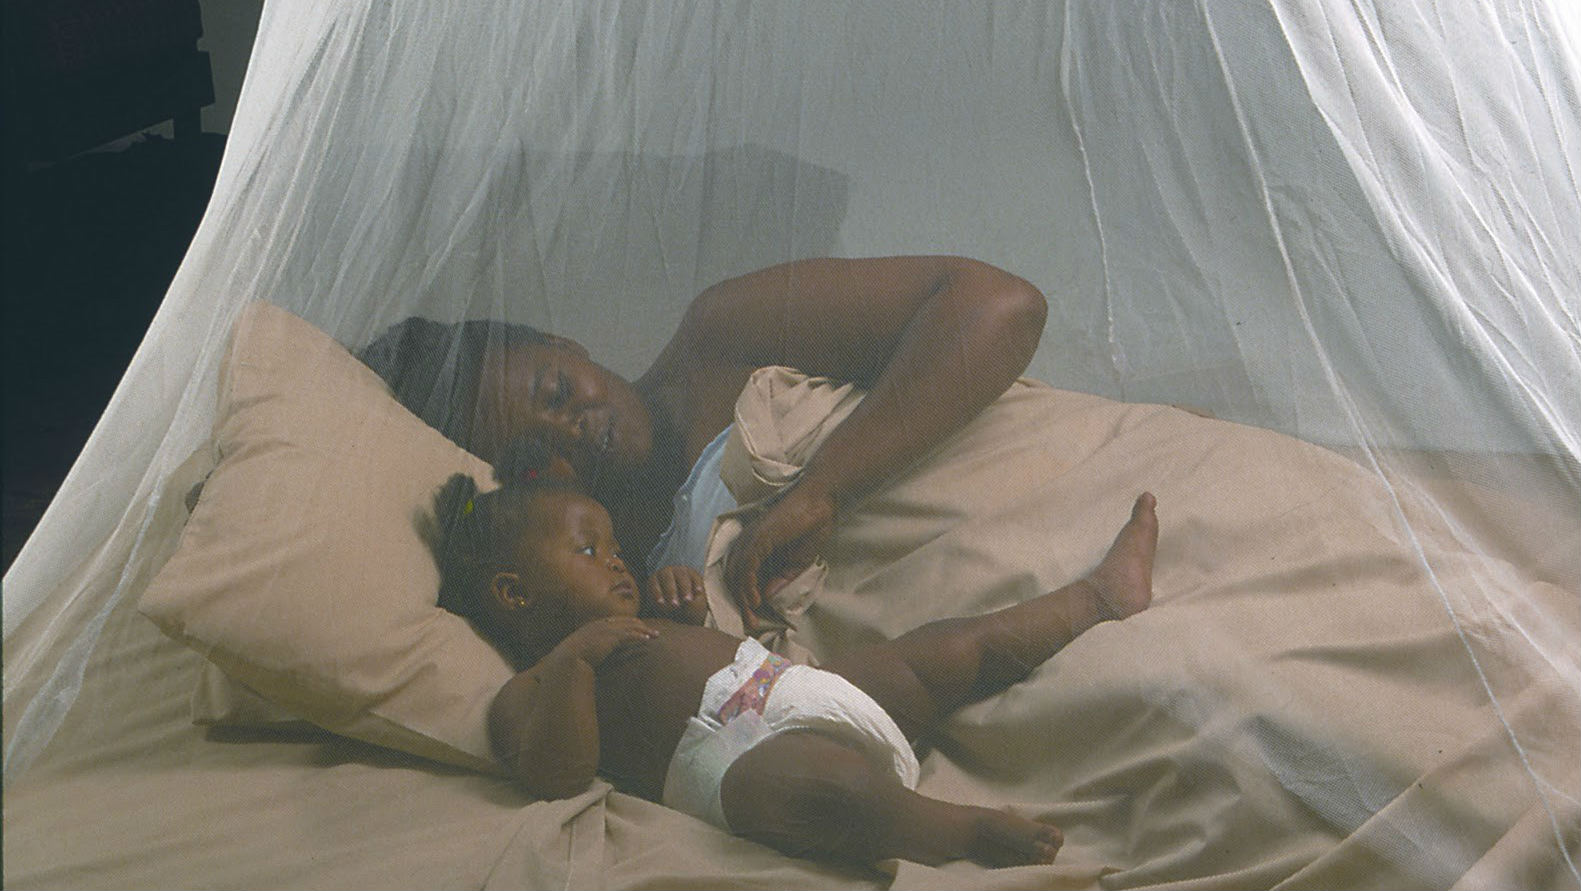
\includegraphics[width=300px]{EU_34351.jpg}%
\newline%
%
Impregnar los mosquiteros con un medicamento antimalaria utilizado con frecuencia en seres humanos podría convertirse en una nueva herramienta para combatir la enfermedad, puesto que ciertos mosquitos se han vuelto resistentes a los insecticidas, según un estudio publicado este miércoles.%
\newline%
%
El uso de insecticidas en los mosquiteros ha sido durante años parte de los recursos recomendados por la Organización Mundial de la Salud (OMS) para prevenir las picaduras de mosquitos portadores de la malaria, también conocida como paludismo.%
\newline%
%
Según un estudio de 2015, se había logrado disminuir en dos tercios las infecciones a nivel mundial desde 2000 con este método.  \newline%
\newline%
Pero cada vez más mosquitos han desarrollado resistencia a los insecticidas hasta ahora utilizados, lo que cuestiona la efectividad de esta estrategia.%
\newline%
%
La OMS advirtió en noviembre sobre el estancamiento en los últimos años de la lucha contra una epidemia que afectó a 219 millones de personas y causó 435.000 muertes en 2017.%
\newline%
%
Un equipo de investigadores de la Universidad de Harvard (Boston, EEUU), diseñó una vía alternativa que no mata a los mosquitos, pero elimina al parásito Plasmodium, responsable de la enfermedad de la que son portadores. \newline%
\newline%
Los científicos reprodujeron en laboratorio una situación similar a la que ocurre cuando un mosquito cae en un mosquitero.%
\newline%
%
Los insectos se alimentaron con sangre contaminada con el parásito y luego fueron puestos en contacto durante seis minutos con una superficie cubierta con una baja dosis de Atovacuona o ATQ, un medicamento contra la malaria.%
\newline%
%
En los seres humanos este medicamento de tipo preventivo mata al parásito e inhibe las funciones mitocondriales. Según el artículo publicado en la revista Nature, se obtuvo el mismo resultado exponiendo a los insectos directamente a la ATQ.%
\newline%
%
"Probamos dos tipos de medicamentos contra el paludismo y esto funcionó muy bien con la ATQ: ¡todos los parásitos fueron eliminados!", explicó Flaminia Catteruccia, profesora de Infectología en Harvard y coautora del estudio.%
\newline%
%
Este método es "seguro para las personas que duermen bajo los mosquiteros y para el medio ambiente", subrayó Catteruccia, y también ha sido eficaz poniendo a los mosquitos en contacto con el medicamento 24 horas antes de ingerir sangre infectada.%
\newline%
%
Según el modelo informático desarrollado por los investigadores, este método "compensaría de manera significativa los efectos sanitarios de la resistencia de los mosquitos a los insecticidas" en la lucha contra la malaria. \newline%
\newline%
Las investigaciones al respecto se encuentran aún en una fase preliminar.%
\newline%
%
\end{document}